
\section{UML MODELS}
\subsection{Use case diagram}
\subsection{Use case Description and sequence diagram}
\subsection{Class Diagram}
\begin{figure}[h]
	\centering
	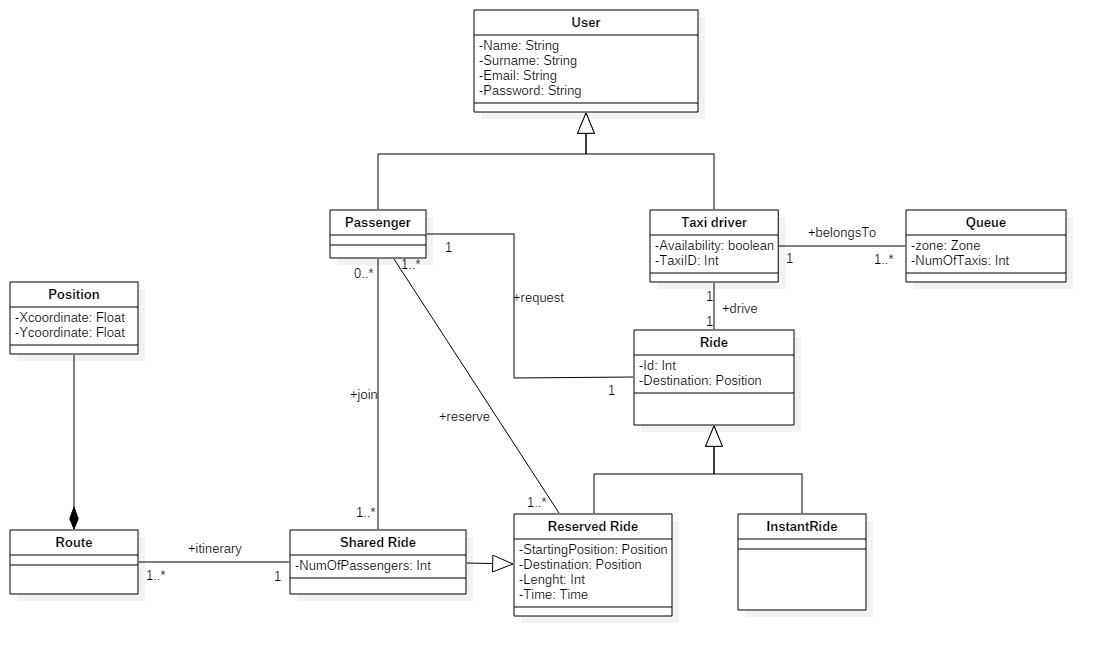
\includegraphics[width=\textwidth+]{class_diagram}
\end{figure}
\newpage
\subsection{State chart diagram}
\begin{enumerate}
	\item User makes a request
	\begin{figure}[h]
		\centering
		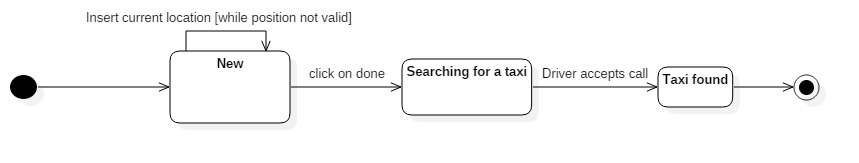
\includegraphics[width=\textwidth+]{Request}
	\end{figure}

	\item User makes a reservation
	\begin{figure}[h]
		\centering
		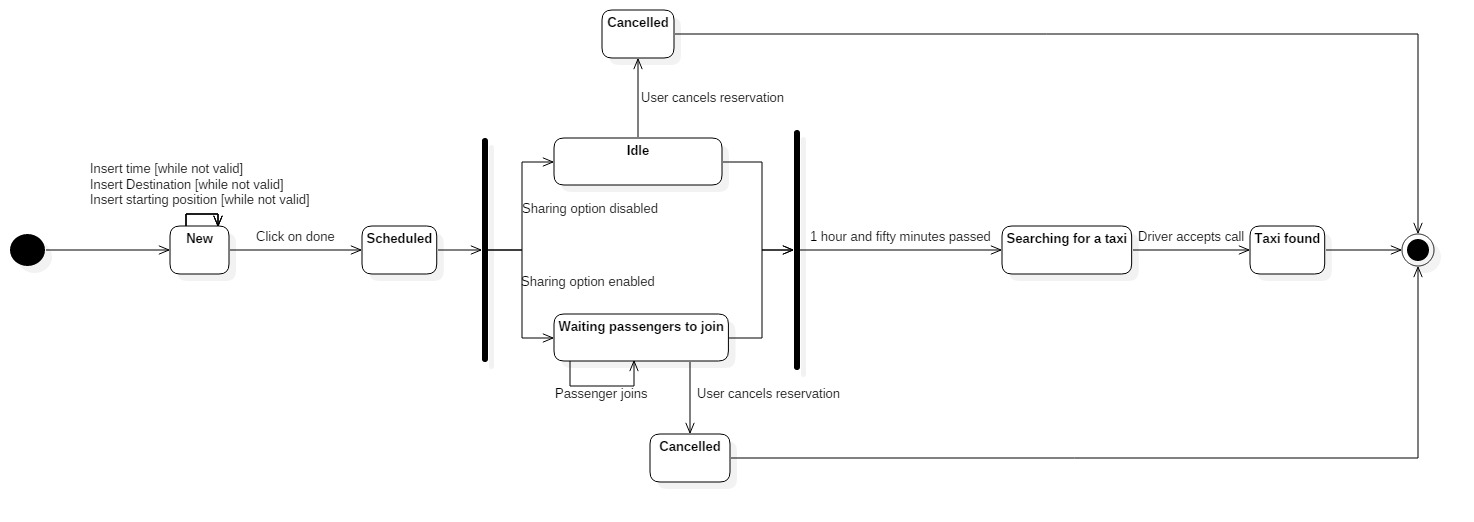
\includegraphics[width=\textwidth+]{reservation}
	\end{figure}
	\newpage
	\item Taxi driver states
	\begin{figure}[h]
		\centering
		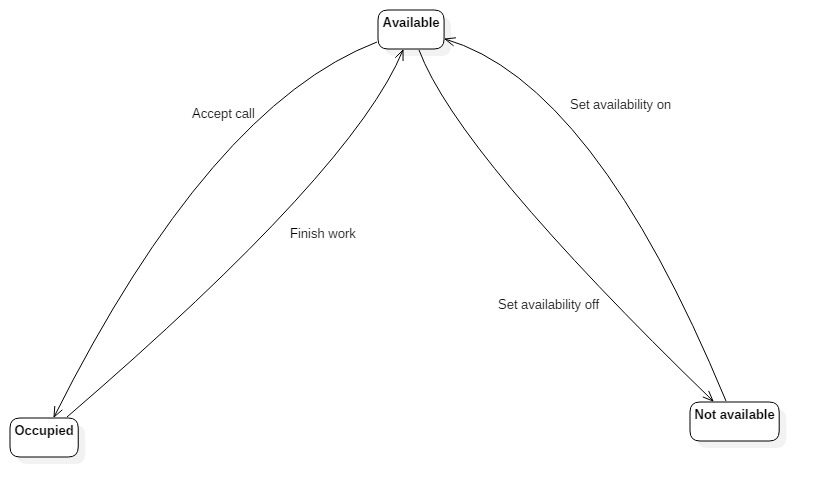
\includegraphics[width=\textwidth+]{taxidriver_statechart}
	\end{figure}
\end{enumerate}